% Ver el archivo config.tex ya que contiene templates de código útil y diferentes operadores matemáticos.
% ***************************************************
% FORMATO.
% ***************************************************
\documentclass[a4paper,12pt]{article}
% Input encoding.
% Idioma.
\usepackage[spanish, es-tabla]{babel}
\usepackage[utf8]{inputenc}
% Ver pagina 92 de "The not so short introduction to Latex" por Tobias Oetiker
% para entender que hacen estos paquetes.
\usepackage{lmodern}
\usepackage[T1]{fontenc}
\usepackage{textcomp}
% Paquete para utilizar el font Times Roman de Adobe por defecto.
\usepackage{mathptmx}
 
%Manejo de márgenes
%Agrega 2cm al ancho por defecto (usado junto con hoffset, no se pierde el centrado)
\addtolength{\textwidth}{2cm}
%Quita 1cm al margen, pero mantiene la relación repecto de cada margen
\addtolength{\hoffset}{-1cm}
\addtolength{\textheight}{2cm}
\addtolength{\voffset}{-1cm}
\setlength{\headheight}{14pt}

% Paquete para manejo de headers y footers.
\usepackage{fancyhdr}
\usepackage{lastpage}
% Determinación del estilo de página (encabezado y pie). Debe ir luego del bloque de manejo de margenes para que
% no haya problemas de dimensiones. Por ejemplo, que el texto quede mas ancho que el encabezado o pie.
\pagestyle{fancy}


% Paquete para manejo de textos en varbatim en varios lugares del documento, por ejemplo en los headers.
\usepackage{fancyvrb}
% Paquete para manejo de boxes de manera mas flexible.
\usepackage{fancybox}

% Para no mostrar el numero de pagina, usar las siguientes dos lineas:
%\thispagestyle{empty}
%\setcounter{savepage}{\thepage}

% Paquete para hacer subrayados, poner textos en color y resaltar texto en color.
% Lo bueno de este paquete es que no tira errores de fullbox como cuando se usa \colorbox{declared-color}{text}.
% El unico problema es que no soporta acentos desde el teclado (tira un error de UTF8). Hay que incluirlos usando \'.
\usepackage{soul}
% Configura el paquete @SOUL para que el resaltado de texto sea rojo. La sintaxis es \hl{text}.
\sethlcolor{red}

% Paquete que deja sangria luego de comenzada una seccion nueva.
%\usepackage{indentfirst}

% Se define una macro para poner double quotes de manera simple. El uso es \quotes{Hello World!}.
\newcommand{\quotes}[1]{``#1''}

% ***************************************************
% MATEMATICA.
% ***************************************************
\usepackage{amsmath}
	% Formato de numeracion de ecuaciones por seccion. Ej. seccion x, ecuacion y: (x.y)
	\numberwithin{equation}{section}
	\numberwithin{figure}{section}
	
% Simbolos matematicos. Por ej. la 'R' de reales, etc...
\usepackage{amssymb}
\usepackage{amsfonts}

\usepackage{mathtools}

% Paquete para arrays de ecuaciones.
\usepackage[retainorgcmds]{IEEEtrantools}
% Unidad imaginaria.
\newcommand{\iu}{{j\mkern1mu}}
% Contador de uso generico.
\newcounter{hipotesis_ct}
\setcounter{hipotesis_ct}{1}

% Operador 'derivada'.
\makeatletter
\providecommand*{\diff}%
{\@ifnextchar^{\DIfF}{\DIfF^{}}}
\def\DIfF^#1{%
	\mathop{\mathrm{\mathstrut d}}%
	\nolimits^{#1}\gobblespace}
\def\gobblespace{%
	\futurelet\diffarg\opspace}
\def\opspace{%
	\let\DiffSpace\!%
	\ifx\diffarg(%
	\let\DiffSpace\relax
	\else
	\ifx\diffarg[%
	\let\DiffSpace\relax
	\else
	\ifx\diffarg\{%
	\let\DiffSpace\relax
	\fi\fi\fi\DiffSpace}

% Uso:
% \pderiv[n]{A}{B}
\providecommand*{\deriv}[3][]{%
	\frac{\diff^{#1}#2}{\diff #3^{#1}}}
\providecommand*{\pderiv}[3][]{%
	\frac{\partial^{#1}#2}%
	{\partial #3^{#1}}}

% Operadores 'valor absoluto' y 'norma'.
% Uso: \abs{123} \norm{123} \abs*{123} \norm*{123}
\DeclarePairedDelimiter\abs{\lvert}{\rvert}%
\DeclarePairedDelimiter\norm{\lVert}{\rVert}%
% Swap the definition of \abs* and \norm*, so that \abs
% and \norm resizes the size of the brackets, and the 
% starred version does not.
\makeatletter
\let\oldabs\abs
\def\abs{\@ifstar{\oldabs}{\oldabs*}}
%
\let\oldnorm\norm
\def\norm{\@ifstar{\oldnorm}{\oldnorm*}}
\makeatother

% Operadores para escribir vectores en negrita directamente.
% Ej:  $\vecbf{v} = 5\vechat{k}$ 
\newcommand{\vecbf}[1]{\mathbf{#1}}
% Operador para escribir en negrita todo lo que tenga hat.
\newcommand{\vechat}[1]{\hat{\mathbf{#1}}}

% ***************************************************
% CODIGO FUENTE.
% ***************************************************
% Paquetes para pseudocodigo.	
\usepackage{lgrind}
\usepackage{algorithm}
\usepackage{algpseudocode}
\makeatletter
\renewcommand{\ALG@name}{Algoritmo}
\renewcommand{\listalgorithmname}{Lista de \ALG@name s}
\algrenewcommand\algorithmicensure{\textbf{Salida:}}
\algrenewcommand\algorithmicrequire{\textbf{Entrada:}}
\algnewcommand{\LineComment}[1]{\State \(\triangleright\) #1}
\makeatother

% Paquete para incluir codigo de MatLab.
\usepackage[numbered,framed]{matlab-prettifier}
% Paquete para control de colores. Ya lo carga 'matlab-prettifier'.
\PassOptionsToPackage{usenames,dvipsnames}{xcolor}

% Fuente: http://en.wikibooks.org/wiki/LaTeX/Colors
\definecolor{Apricot}{RGB}{253,199,130}
\definecolor{Aquamarine}{RGB}{0,181,202}
\definecolor{Bittersweet}{RGB}{192,79,23}
\definecolor{Black}{RGB}{0,0,0}
\definecolor{Blue}{RGB}{0,0,255}
\definecolor{BlueGreen}{RGB}{0,179,184}
\definecolor{BlueViolet}{RGB}{71,57,146}
\definecolor{BrickRed}{RGB}{182,50,28}
\definecolor{Brown}{RGB}{121,37,0}
\definecolor{BurntOrange}{RGB}{247,146,29}
\definecolor{CadetBlue}{RGB}{116,114,154}
\definecolor{CarnationPink}{RGB}{242,130,180}
\definecolor{Cerulean}{RGB}{0,162,227}
\definecolor{CornflowerBlue}{RGB}{65,176,228}
\definecolor{Cyan}{RGB}{0,174,239}
\definecolor{Dandelion}{RGB}{253,188,66}
\definecolor{DarkOrchid}{RGB}{164,83,138}
\definecolor{Emerald}{RGB}{0,169,157}
\definecolor{ForestGreen}{RGB}{0,155,85}
\definecolor{Fuchsia}{RGB}{140,54,140}
\definecolor{Goldenrod}{RGB}{255,223,66}
\definecolor{Gray}{RGB}{148,150,152}
\definecolor{Green}{RGB}{0,166,79}
\definecolor{GreenYellow}{RGB}{223,230,116}
\definecolor{JungleGreen}{RGB}{0,169,154}
\definecolor{Lavender}{RGB}{244,158,196}
\definecolor{LimeGreen}{RGB}{141,199,62}
\definecolor{Magenta}{RGB}{236,0,140}
\definecolor{Mahogany}{RGB}{169,52,31}
\definecolor{Maroon}{RGB}{175,50,53}
\definecolor{Melon}{RGB}{248,158,123}
\definecolor{MidnightBlue}{RGB}{0,103,149}
\definecolor{Mulberry}{RGB}{169,60,147}
\definecolor{NavyBlue}{RGB}{0,103,149}
\definecolor{OliveGreen}{RGB}{60,128,49}
\definecolor{Orange}{RGB}{245,129,55}
\definecolor{OrangeRed}{RGB}{237,19,90}
\definecolor{Orchid}{RGB}{175,114,176}
\definecolor{Peach}{RGB}{247,150,90}
\definecolor{Periwinkle}{RGB}{121,119,184}
\definecolor{PineGreen}{RGB}{0,139,114}
\definecolor{Plum}{RGB}{146,38,143}
\definecolor{ProcessBlue}{RGB}{0,176,240}
\definecolor{Purple}{RGB}{153,71,155}
\definecolor{RawSienna}{RGB}{151,64,6}
\definecolor{Red}{RGB}{237,27,35}
\definecolor{RedOrange}{RGB}{242,96,70}
\definecolor{RedViolet}{RGB}{161,36,107}
\definecolor{Rhodamine}{RGB}{239,85,159}
\definecolor{RoyalBlue}{RGB}{0,113,188}
\definecolor{RoyalPurple}{RGB}{97,63,153}
\definecolor{RubineRed}{RGB}{237,1,125}
\definecolor{Salmon}{RGB}{246,146,137}
\definecolor{SeaGreen}{RGB}{63,188,157}
\definecolor{Sepia}{RGB}{103,24,0}
\definecolor{SkyBlue}{RGB}{70,197,221}
\definecolor{SpringGreen}{RGB}{198,220,103}
\definecolor{Tan}{RGB}{218,157,118}
\definecolor{TealBlue}{RGB}{0,174,179}
\definecolor{Thistle}{RGB}{216,131,183}
\definecolor{Turquoise}{RGB}{0,180,206}
\definecolor{Violet}{RGB}{88,66,155}
\definecolor{VioletRed}{RGB}{239,88,160}
\definecolor{White}{RGB}{255,255,255}
\definecolor{WildStrawberry}{RGB}{238,41,103}
\definecolor{Yellow}{RGB}{255,242,0}
\definecolor{YellowGreen}{RGB}{152,204,112}
\definecolor{YellowOrange}{RGB}{250,162,26}


\lstdefinestyle{StyleMake}{%
	linewidth=\textwidth,%		Define el ancho máximo de una linea de código
	xleftmargin=2.5pt,%				Margen izquierdo
	xrightmargin=2.5pt,%				Margen derecho
	breaklines=true,%				Que corte lineas largas
	numbers=left,%			Que haya números a la izquierda (número de linea)
	numberstyle=\scriptsize,%		Formato de los números de linea
	stepnumber=1,%					Que avancen de a 1 (ver todos los números)
	numbersep=10pt,%					La separación de los números del código
	tabsize=4,showtabs=false,%		Los TABS son 4 espacios, y no se ven
	extendedchars=true,%			Se permiten caracteres extendidos
	basicstyle=\ttfamily\small,%	Estilo básico de la tipografía del código
	commentstyle=\color{Blue},%		Color de los comentarios
	showstringspaces=false,%		Los espacios no se ven de forma especial
	stringstyle=\color{BrickRed},%	Estilo de las cadenas
	keywordstyle=\color{ForestGreen},%	Estilo de las palabras reservadas
	morekeywords=[1]{g++,-Wall,-pedantic},%	Definición de más palabras reservadas
	deletekeywords={rm,-rf,*.o},%
	keywords=[2]{rm,-rf,*.o},%
	keywordstyle=[2]{\color{BurntOrange}},%	2do grupo de palabras reservadas
	directives={CC,CFLAGS,OUTPUT},%
	directivestyle=\color{NavyBlue},%	Estilo de directivas
	keywords=[3]{CC,CFLAGS,OUTPUT},%
	keywordstyle=[3]{\color{MidnightBlue}},%3er grupo de palabras reservadas
	morecomment=[s][\color{Blue}]{/*}{*/}%	Definición de estilo de comentario
}

\lstdefinestyle{StyleC}{%
	linewidth=\textwidth,%		Define el ancho máximo de una linea de código
	xleftmargin=2.5pt,%				Margen izquierdo
	xrightmargin=2.5pt,%				Margen derecho
	breaklines=true,%				Que corte lineas largas
	numbers=left,%			Que haya números a la izquierda (número de linea)
	numberstyle=\scriptsize,%		Formato de los números de linea
	stepnumber=1,%					Que avancen de a 1 (ver todos los números)
	numbersep=10pt,%					La separación de los números del código
	tabsize=4,showtabs=false,%		Los TABS son 4 espacios, y no se ven
	extendedchars=true,%			Se permiten caracteres extendidos
	basicstyle=\ttfamily\small,%	Estilo básico de la tipografía del código
	commentstyle=\color{Blue},%		Color de los comentarios
	showstringspaces=false,%		Los espacios no se ven de forma especial
	stringstyle=\color{BrickRed},%	Estilo de las cadenas
	keywordstyle=\color{ForestGreen},%	Estilo de las palabras reservadas
	morekeywords=[1]{size_t,ssize_t},%	Definición de más palabras reservadas
	deletekeywords={typedef,enum,do,while,if,else,for,case,default,switch,break,continue},%
	keywords=[2]{typedef,enum,do,while,if,else,for,case,default,switch,break,continue,EXIT_SUCCESS,EXIT_FAILURE},%
	keywordstyle=[2]{\color{BurntOrange}},%	2do grupo de palabras reservadas
	directives={define,undef,include,if,else,ifndef,ifdef,elif,endif},%
	directivestyle=\color{NavyBlue},%		Estilo de directivas
	keywords=[3]{define,undef,include,if,else,ifndef,ifdef,elif,endif},%
	keywordstyle=[3]{\color{MidnightBlue}},%3er grupo de palabras reservadas
	morecomment=[s][\color{Blue}]{/*}{*/}%	Definición de estilo de comentario
}

\lstnewenvironment{terminalblock}{%
	\lstset{style=StyleC}}{}

\lstset{
	literate={ö}{{\"o}}1
	{ä}{{\"a}}1
	{ü}{{\"u}}1
	{á}{{\'a}}1
	{Á}{{\'A}}1
	{é}{{\'e}}1
	{É}{{\'E}}1
	{í}{{\'i}}1
	{Í}{{\'I}}1
	{ñ}{{\~n}}1
	{ó}{{\'o}}1
	{Ó}{{\'O}}1
	{ú}{{\'u}}1
	{Ú}{{\'U}}1
}

\definecolor{listinggray}{gray}{0.9}
\definecolor{lbcolor}{rgb}{0.9,0.9,0.9}
% http://tex.stackexchange.com/questions/44282/multiline-comment
\newcommand{\comment}[1]{}

\lstset{
	backgroundcolor=\color{lbcolor},
	tabsize=4,    
	language=[GNU]C++,
	basicstyle=\scriptsize,
	upquote=true,
	aboveskip={1.5\baselineskip},
	columns=fixed,
	showstringspaces=false,
	extendedchars=false,
	breaklines=true,
	prebreak = \raisebox{0ex}[0ex][0ex]{\ensuremath{\hookleftarrow}},
	frame=single,
	numbers=left,
	showtabs=false,
	showspaces=false,
	showstringspaces=false,
	identifierstyle=\ttfamily,
	keywordstyle=\color[rgb]{0,0,1},
	commentstyle=\color[rgb]{0.026,0.112,0.095},
	stringstyle=\color[rgb]{0.627,0.126,0.941},
	numberstyle=\color[rgb]{0.205, 0.142, 0.73},
}

\lstset{
	backgroundcolor=\color{lbcolor},
	tabsize=4,
	language=C++,
	captionpos=b,
	tabsize=3,
	frame=lines,
	numbers=left,
	numberstyle=\tiny,
	numbersep=5pt,
	breaklines=true,
	showstringspaces=false,
	basicstyle=\footnotesize,
	keywordstyle=\color[rgb]{0,0,1},
	commentstyle=\color[rgb]{0.026,0.112,0.095},
	stringstyle=\color{red},
}
% ***************************************************
% GRAFICOS.
% ***************************************************
	% Paquete para mejorar la interfaz con objetos flotantes, como los graficos.
	\usepackage{float}
	\usepackage{graphicx}
	% Paquetes para tener mayor flexibilidad cuando se utilizan titulos para figuras, etc...
	\usepackage{caption}
	\usepackage{subcaption}
	\usepackage{epstopdf}

% ***************************************************
% TABLAS.
% ***************************************************
% Paquetes para manejo de tablas.
\usepackage{booktabs}
\usepackage{multirow}

% ***************************************************
% MISC.
% ***************************************************
%\usepackage{draftwatermark}
%\SetWatermarkLightness{0.95}
%\SetWatermarkScale{0.8}
%\SetWatermarkText{BORRADOR}

% This pack­age sim­pli­fies the in­clu­sion of ex­ter­nal multi-page PDF doc­u­ments in LaTeX doc­u­ments. 
\usepackage{pdfpages}
\setboolean{@twoside}{false}

% Unidades del SI
\usepackage[per-mode=symbol]{siunitx}

% Adds bibliography section to the TOC.
\usepackage[nottoc,notlot,notlof]{tocbibind}

% ***************************************************
% TIKZ.
% ***************************************************
%\usepackage{tikz}
%\usetikzlibrary{calc,fadings,decorations.pathreplacing,shapes,arrows}
%\usetikzlibrary{decorations.pathmorphing} % for snake lines
%\usetikzlibrary{matrix} % for block alignment
%\usetikzlibrary{arrows} % for arrow heads
%\usetikzlibrary{calc} % for manimulation of coordinates
%
%% TikZ styles for drawing
%\tikzstyle{block} = [draw,rectangle,thick,minimum height=2em,minimum width=2em]
%\tikzstyle{sum} = [draw,circle,inner sep=0mm,minimum size=2mm]
%\tikzstyle{connector} = [->,thick]
%\tikzstyle{line} = [thick]
%\tikzstyle{branch} = [circle,inner sep=0pt,minimum size=1mm,fill=black,draw=black]
%\tikzstyle{guide} = []
%\tikzstyle{snakeline} = [connector, decorate, decoration={pre length=0.2cm,post length=0.2cm, snake, amplitude=.4mm,segment length=2mm},thick, magenta, ->]
%
%\renewcommand{\vec}[1]{\ensuremath{\boldsymbol{#1}}} % bold vectors
%\def \myneq {\skew{-2}\not =} % \neq alone skews the dash
%%% helper macros
%\newcommand\pgfmathsinandcos[3]{%
%	\pgfmathsetmacro#1{sin(#3)}%
%	\pgfmathsetmacro#2{cos(#3)}%
%}
%\newcommand\LongitudePlane[3][current plane]{%
%	\pgfmathsinandcos\sinEl\cosEl{#2} % elevation
%	\pgfmathsinandcos\sint\cost{#3} % azimuth
%	\tikzset{#1/.estyle={cm={\cost,\sint*\sinEl,0,\cosEl,(0,0)}}}
%}
%\newcommand\LatitudePlane[3][current plane]{%
%	\pgfmathsinandcos\sinEl\cosEl{#2} % elevation
%	\pgfmathsinandcos\sint\cost{#3} % latitude
%	\pgfmathsetmacro\yshift{\cosEl*\sint}
%	\tikzset{#1/.estyle={cm={\cost,0,0,\cost*\sinEl,(0,\yshift)}}} %
%}
%\newcommand\DrawLongitudeCircle[2][1]{
%	\LongitudePlane{\angEl}{#2}
%	\tikzset{current plane/.prefix style={scale=#1}}
%	% angle of "visibility"
%	\pgfmathsetmacro\angVis{atan(sin(#2)*cos(\angEl)/sin(\angEl))} %
%	\draw[current plane] (\angVis:1) arc (\angVis:\angVis+180:1);
%	\draw[current plane,dashed] (\angVis-180:1) arc (\angVis-180:\angVis:1);
%}
%\newcommand\DrawLatitudeCircle[2][1]{
%	\LatitudePlane{\angEl}{#2}
%	\tikzset{current plane/.prefix style={scale=#1}}
%	\pgfmathsetmacro\sinVis{sin(#2)/cos(#2)*sin(\angEl)/cos(\angEl)}
%	% angle of "visibility"
%	\pgfmathsetmacro\angVis{asin(min(1,max(\sinVis,-1)))}
%	\draw[current plane] (\angVis:1) arc (\angVis:-\angVis-180:1);
%	\draw[current plane,dashed] (180-\angVis:1) arc (180-\angVis:\angVis:1);
%}
%
%%% document-wide tikz options and styles
%\tikzset{%
%	>=latex, % option for nice arrows
%	inner sep=0pt,%
%	outer sep=2pt,%
%	mark coordinate/.style={inner sep=0pt,outer sep=0pt,minimum size=3pt,
%		fill=black,circle}%
%}

% ***************************************************
% HIPERTEXTO.
% ***************************************************
% Paquete para utilizar hipertexto (tiene que ser siempre el ultimo paquete que se carga).
% Todos los links, referencias, etc...pasan a ser hipertextos.
% Setup del paquete de hipertexto.
\usepackage[pdftex,breaklinks]{hyperref}
	\hypersetup{a4paper,
				% Muestra el titulo en el maro superior de la ventana del visor de pdf
				pdfdisplaydoctitle=true,
				% Al encender esta funcion, ya nohay recuadros feos alrededor de los links 	
				colorlinks=true,
				% Color cuando se escribe una URL.   
				urlcolor = black,
				%Para que el link a nuevos pdf, no se abran en la misma ventana 		
				pdfnewwindow=true,
				% Color para links internos
				linkcolor=black,
				% Color para links a Bibliografia
				citecolor=black,
				% Color para links a archivos
       			filecolor=black,
				pdftitle={Modelo informe},
				pdfauthor={husain}
			}

% ***************************************************			
% GLOSARIO.
% ***************************************************
% Glosario. Debe cargarse después del paquete "hyperref", como excepción.
%\include{./misc/glossary}

% ***************************************************			
% ALGUNOS TEMPLATES DE CODIGO UTIL.
% ***************************************************

% *********************************************************************************
% Si incluyo figuras de MatLab, no conviene que se guarden maximizadas.
%\begin{figure}[!ht]
%	\centering
%	\includegraphics[scale=0.9]{includes/ex1_N5.eps}
%	\caption{Submuestreo con $N=5$ con $M=3$ y $M=6$}
%	\label{ex1_N5}
%\end{figure}
% *********************************************************************************
%\begin{figure}[H]
%	\centering
%	\begin{subfigure}[c]{0.3\textwidth}
%		\includegraphics[scale=0.06]{./includes/cover/Logo_UBA.eps}
%	\end{subfigure}
%	\begin{subfigure}[c]{0.3\textwidth}
%		\includegraphics[scale=0.5]{./includes/cover/Logo_FIUBA.eps}
%	\end{subfigure}
%\end{figure}
% *********************************************************************************
%\begin{IEEEeqnarray}{rCl}
%\IEEEyesnumber\label{ec_ex1_relaciones} \IEEEyessubnumber*
%x\left( n \right)  \  &=& \, x\left( n + k \, N \right) \label{ec_ex1_x}\\
%y\left( n \right)  \, &=& \, y\left( n + l \, L \right) \label{ec_ex1_y}\\
%y\left( n \right)  \, &=& \, x\left( M \, n \right) \label{ec_ex1_downsampling}
%\end{IEEEeqnarray}
%\begin{IEEEeqnarray}{CC}
%	\IEEEyesnumber\label{eq:both} \IEEEyessubnumber*
%	bla bla & blub blub \label{eq:sub1}\\
%	bla bla & bla bla  \label{eq:sub2}
%\end{IEEEeqnarray}
%where the set of equations \eqref{eq:sub1} and \eqref{eq:sub2}
%is referred to as \eqref{eq:both}.
%\begin{align}
%N_{x,sk} &= k_{sk}\left(\frac{t_{sk}}{b_{sk}}\right)^{2}\bar{Et}\nonumber\\
%N_{x,st} &= k_{st}\left(\frac{t_{st}}{b_{st}}\right)^{2}\bar{Et}
%\end{align}
% *********************************************************************************
%\begin{equation}
%\begin{cases}
%H\left( z \right) &= \sum_{l=0}^{M-1} \, z^{-l} \, E_l\left( z^M \right) \\
%E_l\left( z \right) &= \sum_{n=-\infty}^{+\infty} \, e_l \left( n \right) \, z^{-n} \\
%e_l\left( n \right) &= h\left(n\,M + l\right) \quad 0 \leq l \leq M-1
%\end{cases}
%\end{equation}
% *********************************************************************************
%\begin{equation}
%\mathbf{R}_x\left(\phi\right) = 
%\begin{bmatrix}
%1 & 0 & 0 \\
%0 & \cos \left(\phi\right) & \sin \left(\phi\right) \\
%0 & -\sin \left(\phi\right) & \cos \left(\phi\right) \\
%\end{bmatrix}
%\end{equation}
% *********************************************************************************
%\begin{algorithm}[!ht]
%\caption{Pseudocódigo del algoritmo euclídeo extendido}\label{alg_euc_ex}
%\begin{algorithmic}[1]
%\Require $H_0\left(z\right)$ y $H_1\left(z\right)$ coprimos
%\Ensure  $F_0\left(z\right)$ y $F_1\left(z\right)$ tales que $H_0\left(z\right)\cdot F_0\left(z\right)+H_1\left(z\right)\cdot F_1\left(z\right) = c$, con $c\neq0$. Además, $gr\left(F_0\right) < gr\left(H_1\right) - gr\left(g\right)$ y $gr\left(F_1\right) < gr\left(H_0\right) - gr\left(g\right)$.
%\Statex
%\Procedure{extEuclidean}{}
%\Statex
%\State Inicialización.
%\Statex
%\State $r_0=H_0 \quad r_1=H_1 \quad s_0=1 \quad s_1=0 \quad t_0=0 \quad t_1=1 \quad i=1$
%\Statex
%\While {$r_i\neq0 \quad\wedge\quad gr\left(r_{i+1}\right)\geqslant gr\left(r_i\right)$:}
%\Statex
%\State $q \leftarrow$ Cociente de $r_{i-1}/r_i$
%\Statex
%\State $r_{i+1} = r_{i-1} - q\,r_i$
%\Statex
%\State $s_{i+1} = s_{i-1} - q\,s_i$
%\Statex
%\State $t_{i+1} = t_{i-1} - q\,t_i$
%\Statex
%\State $i = i+1$
%\EndWhile
%\Statex
%\State $F_0\left(z\right) = s_{i-1} \quad F_1\left(z\right)=t_{i-1} \quad g=r_{i-1}$
%\EndProcedure
%\end{algorithmic}
%\end{algorithm}
% *********************************************************************************
%\begin{table}
%	\caption{A badly formatted table}
%	\centering
%	\label{table:bad_table}
%	\begin{tabular}{|l|c|c|c|c|}
%		\hline 
%		& \multicolumn{2}{c}{Species I} & \multicolumn{2}{c|}{Species II} \\ 
%		\hline
%		Dental measurement  & mean & SD  & mean & SD  \\ \hline 
%		\hline
%		I1MD & 6.23 & 0.91 & 5.2  & 0.7  \\
%		\hline 
%		I1LL & 7.48 & 0.56 & 8.7  & 0.71 \\
%		\hline 
%		I2MD & 3.99 & 0.63 & 4.22 & 0.54 \\
%		\hline 
%		I2LL & 6.81 & 0.02 & 6.66 & 0.01 \\
%		\hline 
%		CMD & 13.47 & 0.09 & 10.55 & 0.05 \\
%		\hline 
%		CBL & 11.88 & 0.05 & 13.11 & 0.04\\ 
%		\hline 
%	\end{tabular}
%\end{table}
% *********************************************************************************
%\begin{table}
%	\caption{A nice looking table}
%	\centering
%	\label{table:nice_table}
%	\begin{tabular}{l c c c c}
%		\hline 
%		\multirow{2}{*}{Dental measurement} & \multicolumn{2}{c}{Species I} & \multicolumn{2}{c}{Species II} \\ 
%		\cline{2-5}
%		& mean & SD  & mean & SD  \\ 
%		\hline
%		I1MD & 6.23 & 0.91 & 5.2  & 0.7  \\
%		
%		I1LL & 7.48 & 0.56 & 8.7  & 0.71 \\
%		
%		I2MD & 3.99 & 0.63 & 4.22 & 0.54 \\
%		
%		I2LL & 6.81 & 0.02 & 6.66 & 0.01 \\
%		
%		CMD & 13.47 & 0.09 & 10.55 & 0.05 \\
%		
%		CBL & 11.88 & 0.05 & 13.11 & 0.04\\ 
%		\hline 
%	\end{tabular}
%\end{table}
% *********************************************************************************
%\begin{table}
%	\caption{Even better looking table using booktabs}
%	\centering
%	\label{table:good_table}
%	\begin{tabular}{l c c c c}
%		\toprule
%		\multirow{2}{*}{Dental measurement} & \multicolumn{2}{c}{Species I} & \multicolumn{2}{c}{Species II} \\ 
%		\cmidrule{2-5}
%		& mean & SD  & mean & SD  \\ 
%		\midrule
%		I1MD & 6.23 & 0.91 & 5.2  & 0.7  \\
%		
%		I1LL & 7.48 & 0.56 & 8.7  & 0.71 \\
%		
%		I2MD & 3.99 & 0.63 & 4.22 & 0.54 \\
%		
%		I2LL & 6.81 & 0.02 & 6.66 & 0.01 \\
%		
%		CMD & 13.47 & 0.09 & 10.55 & 0.05 \\
%		
%		CBL & 11.88 & 0.05 & 13.11 & 0.04\\ 
%		\bottomrule
%	\end{tabular}
%\end{table}
% *********************************************************************************
%\begin{table}[htbp]
%	\centering
%	\caption{Primeros 40 coeficientes correspondientes a la Teoría de Nutación IAU-1980.}
%	\begin{tabular}{cccccccccc}
%		\toprule
%		\multicolumn{1}{c}{Coeficiente} & \multicolumn{1}{c}{$p_l$} & \multicolumn{1}{c}{$p_l'$} & \multicolumn{1}{c}{$p_F$} & \multicolumn{1}{c}{$p_D$} & \multicolumn{1}{c}{$p_\Omega$} & \multicolumn{1}{c}{$\Delta \hat{\psi} \left[0.001''\right]$} & \multicolumn{1}{c}{$\Delta \hat{\psi}_T\left[0.001''\right]$} & \multicolumn{1}{c}{$\Delta \hat{\varepsilon}\left[0.001''\right]$} & \multicolumn{1}{c}{$\Delta \hat{\varepsilon}_T\left[0.001''\right]$} \\
%		\midrule
%		1     & 0     & 0     & 0     & 0     & 1     & -1719960 & -1742 & 920250 & 89 \\
%		2     & 0     & 0     & 0     & 0     & 2     & 20620 & 2     & -8950 & 5 \\
%		3     & -2    & 0     & 2     & 0     & 1     & 460   & 0     & -240  & 0 \\
%		4     & 2     & 0     & -2    & 0     & 0     & 110   & 0     & 0     & 0 \\
%		5     & -2    & 0     & 2     & 0     & 2     & -30   & 0     & 10    & 0 \\
%		6     & 1     & -1    & 0     & -1    & 0     & -30   & 0     & 0     & 0 \\
%		7     & 0     & -2    & 2     & -2    & 1     & -20   & 0     & 10    & 0 \\
%		8     & 2     & 0     & -2    & 0     & 1     & 10    & 0     & 0     & 0 \\
%		9     & 0     & 0     & 2     & -2    & 2     & -131870 & -16   & 57360 & -31 \\
%		10    & 0     & 1     & 0     & 0     & 0     & 14260 & -34   & 540   & -1 \\
%		11    & 0     & 1     & 2     & -2    & 2     & -5170 & 12    & 2240  & -6 \\
%		12    & 0     & -1    & 2     & -2    & 2     & 2170  & -5    & -950  & 3 \\
%		13    & 0     & 0     & 2     & -2    & 1     & 1290  & 1     & -700  & 0 \\
%		14    & 2     & 0     & 0     & -2    & 0     & 480   & 0     & 10    & 0 \\
%		15    & 0     & 0     & 2     & -2    & 0     & -220  & 0     & 0     & 0 \\
%		16    & 0     & 2     & 0     & 0     & 0     & 170   & -1    & 0     & 0 \\
%		17    & 0     & 1     & 0     & 0     & 1     & -150  & 0     & 90    & 0 \\
%		18    & 0     & 2     & 2     & -2    & 2     & -160  & 1     & 70    & 0 \\
%		19    & 0     & -1    & 0     & 0     & 1     & -120  & 0     & 60    & 0 \\
%		20    & -2    & 0     & 0     & 2     & 1     & -60   & 0     & 30    & 0 \\
%		21    & 0     & -1    & 2     & -2    & 1     & -50   & 0     & 30    & 0 \\
%		22    & 2     & 0     & 0     & -2    & 1     & 40    & 0     & -20   & 0 \\
%		23    & 0     & 1     & 2     & -2    & 1     & 40    & 0     & -20   & 0 \\
%		24    & 1     & 0     & 0     & -1    & 0     & -40   & 0     & 0     & 0 \\
%		25    & 2     & 1     & 0     & -2    & 0     & 10    & 0     & 0     & 0 \\
%		26    & 0     & 0     & -2    & 2     & 1     & 10    & 0     & 0     & 0 \\
%		27    & 0     & 1     & -2    & 2     & 0     & -10   & 0     & 0     & 0 \\
%		28    & 0     & 1     & 0     & 0     & 2     & 10    & 0     & 0     & 0 \\
%		29    & -1    & 0     & 0     & 1     & 1     & 10    & 0     & 0     & 0 \\
%		30    & 0     & 1     & 2     & -2    & 0     & -10   & 0     & 0     & 0 \\
%		31    & 0     & 0     & 2     & 0     & 2     & -22740 & -2    & 9770  & -5 \\
%		32    & 1     & 0     & 0     & 0     & 0     & 7120  & 1     & -70   & 0 \\
%		33    & 0     & 0     & 2     & 0     & 1     & -3860 & -4    & 2000  & 0 \\
%		34    & 1     & 0     & 2     & 0     & 2     & -3010 & 0     & 1290  & -1 \\
%		35    & 1     & 0     & 0     & -2    & 0     & -1580 & 0     & -10   & 0 \\
%		36    & -1    & 0     & 2     & 0     & 2     & 1230  & 0     & -530  & 0 \\
%		37    & 0     & 0     & 0     & 2     & 0     & 630   & 0     & -20   & 0 \\
%		38    & 1     & 0     & 0     & 0     & 1     & 630   & 1     & -330  & 0 \\
%		39    & -1    & 0     & 0     & 0     & 1     & -580  & -1    & 320   & 0 \\
%		40    & -1    & 0     & 2     & 2     & 2     & -590  & 0     & 260   & 0 \\
%		\bottomrule
%	\end{tabular}%
%	\label{table:coefs_nut}
%\end{table}%
% *********************************************************************************
% \ang{23.43929111}
% \ang{;;46.8150}
% $\pm \SI{0.9}{\second}$
% \SI{1e-22}{}
% ...utilizando mediciones en tierra de $F_{\SI{10.7}{}}$: Al dejar vacío el segundo 
% argumento, lo que hace es usar el formato numérico SI, y no el local. O sea, aparece 
% "10.7" en vez de "10,7".
%
% *********************************************************************************
%% This bit allows you to either specify only the files which you wish to
%% process, or `all' to process all files which you \include.
%% Krishna Sethuraman (1990).
%
%\typein [\files]{Enter file names to process, (chap1,chap2 ...), or `all' to process all files:}
%\def\all{all}
%\ifx\files\all \typeout{Including all files.} \else \typeout{Including only \files.} \includeonly{\files} \fi
% *********************************************************************************
% Ignacio Santiago Husain Cerruti - 2020.
% *********************************************************************************

% Especificación del encabezado y pie de página.
\fancyhf{}
\lhead{\small TP1 [1C2022]}
\chead{}
\rhead{\small [75.12] Analisis Numérico}
\rfoot{}
\cfoot{Página {\thepage} de \pageref{LastPage}}
\lfoot{}
\renewcommand{\thesubsection}{\thesection.\alph{subsection}}
%-----------------------------------%
%									%
%		Comienzo del documento		%
%									%
%-----------------------------------%
\begin{document}
%-----------------------------------%
%									%
%			Caratula				%
%									%
%-----------------------------------%
\pagestyle{fancy}
\begin{titlepage}
	\newcommand{\HRule}{\rule{\linewidth}{0.5mm}} % Defines a new command for horizontal lines, change thickness here
	\center % Centre everything on the page
	
	\thispagestyle{empty}
	\begin{center}
		
\includegraphics[scale=0.9]{includes/banner_fiuba.pdf}\\
	\end{center}
	
 	\vspace*{\stretch{1}}
	
	\textsc{\Large \textsc{[75.12] Análisis Numérico}}\\[0.3cm]
	\textsc{\Large \textsc{Trabajo Práctico 1}}\\[0.3cm]
	\textsc{\large 1\textsuperscript{er} Cuatrimestre 2022}\\[0.25cm]
	
	\HRule\\[0.2cm]
	{\large\bfseries Búsqueda de raíces e interpolación}\\[0.2cm]
	\HRule\\[0.2cm]
	
	\begin{tabbing}
		\hspace{2cm}\=\+
		\underline{AUTOR}\hspace{-1cm}\=\+\hspace{1cm}\=\hspace{6cm}\=\\[0.2cm]
		
		Sanchez Fernandez De La Vega, Manuel.	\>\>- \#107951\\
		\>\footnotesize{$<$msanchezf@fi.uba.ar$>$}\\
		Ugarte, Matin.	\>\>- \#107870\\
		\>\footnotesize{$<$mugarte@fi.uba.ar$>$}\\
		Shih, Ian.	\>\>- \#100.000\\
		\>\footnotesize{$<$ishih@fi.uba.ar$>$}\\
		Rodriguez Justo, Ignacio.	\>\>- \#100.000\\
        \>\footnotesize{$<$irodriguezj@fi.uba.ar$>$}\\
        
        \\
        
		\<\underline{CÁTEDRA}\\[0.2cm]
		Myriam Sassano \\
		María Agustina Turano \\
		Ezequiel García \\
		Ramiro Vera \\
		Santiago Husain \\[0.2cm]
		
		 \\
		
		\<\underline{FECHA DE ENTREGA}\>\>\> 29 de junio de 2022
		\\[0.2cm]
		\<\underline{CALIFICACIÓN}\>\>\> 
		\\[0.2cm]
		
	\end{tabbing}
	
	
 	\vspace*{\stretch{1}}
	
	
\end{titlepage}

%-----------------------------------%
%									%
%			Indice					%
%									%
%-----------------------------------%
\clearpage

\tableofcontents							

\clearpage

%-------------------------------%
%								%
%	Seccion: Objetivos			%
%								%
%-------------------------------%
\clearpage
\section{Objetivos}
El presente trabajo tiene los siguientes objetivos:
\begin{itemize}
	\item Modelar .....
	\item Implementar y validar algoritmos ...
	\item Modelar y simular ...
\end{itemize}

%-------------------------------%
%								%
%	Seccion: Ejercicios			%
%								%
%-------------------------------%
\section{Ejercicio 1}

\subsection{}
El problema se basa en encontrar la cantidad minima de acero de calidad a producir tal que sea rentable, alcanzando los \$25000 de contribución mensual y al mismo tiempo se fabrique por lo menos 827 kilogramos de este producto para que se justifique el encendido de la maquina.

La rentabilidad esta dada por la ecuacion: 
\begin{center}$0.001 \cdot x \cdot (x-1000)^2$.\end{center}

\begin{figure}[!ht]
	\centering
	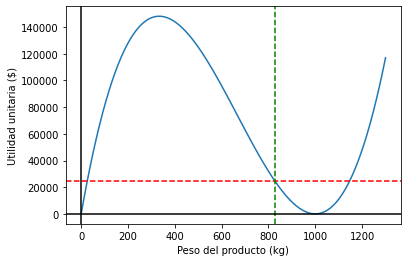
\includegraphics[scale=0.8]{graficos/grafico_del_problema_1.png}
	\caption{Gráfico de la utilidad unitaria en función del peso (azul). La barra verde indica los 827 kilogramos y la roja indica los \$25000} \label{grafico_del_problema_1}
\end{figure}


Por lo tanto, para resolver lo solicitado se puede igualar la expresión anterior a 25000

\begin{center}$0.001 \cdot x \cdot (x-1000)^2 = 25000$\end{center}
\begin{center}$0.001 \cdot x \cdot (x-1000)^2 - 25000 = 0$\end{center}

Como se puede observar, ahora el problema consiste en hallar la raiz de:  

\begin{center}$f(x) = 0.001 \cdot x \cdot (x-1000)^2 - 25000$,\hspace{10mm} $x > 827$\end{center}

\begin{figure}[!ht]
	\centering
	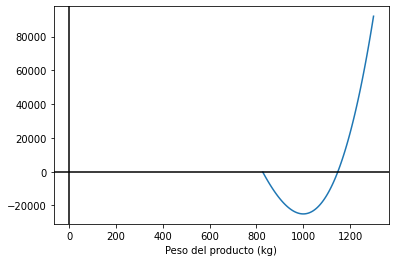
\includegraphics[scale=0.8]{graficos/grafico_del_problema_1_planteo_para_raices.png}
	\caption{Gráfico de la funcion f(x) en azul} \label{planteo_de_raices_problema_1}
\end{figure}

Comenzando con el método de bisección, establecemos un intervalo a partir de observar el gráfico anterior. Este puede ser [$a_0$, $b_0$] siendo $a_0 = 827$ y $b_0 = 1200$.

\begin{figure}[!ht]
	\centering
	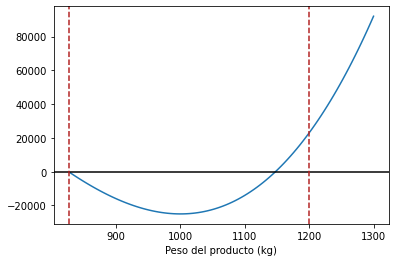
\includegraphics[scale=0.8]{graficos/zoom_en_intervalo_biseccion.png}
	\caption{Gráfico del intervalo establecido} \label{zoom_en_intervalo_biseccion}
\end{figure}

Tenemos que:
\begin{itemize}
    \item $f(a) = -248.717 < 0 $
    \item $f(b) = 23000 > 0 $
\end{itemize}

Graficamente podemos ver que existe una raiz. De otro modo, por teorema de bolzano, verificamos que:
\begin{center} $f(a_0) \cdot f(b_0) < 0 \implies$ Existe una raiz en el intervalo \end{center}

Para hallar la semilla r0:

\begin{center}$r_0 = \frac{827 + 1200}{2} = 1013.5 $\end{center}

Para corroborar si esta es la raiz exacta, se evalúa el resultado en la función

\begin{center}$f(1013.5) \approx -24815.28963 \neq 0 $\end{center}

Como esta no es la raiz, hay que evaluar la funcion en los extremos del intervalo verificando que:


\begin{equation}
        a_{n+1} =
        \begin{cases}{}
            a_n, &\text{$f(a_n) \cdot f(r_n) < 0$}\\
            r_n, &\text{$f(a_n) \cdot f(r_n) > 0$}
        \end{cases}.
\end{equation}

\begin{equation}
        b_{n+1} =
        \begin{cases}{}
            b_n, &\text{$f(b_n) \cdot f(r_n) < 0$}\\
            r_n, &\text{$f(b_n) \cdot f(r_n) > 0$}
        \end{cases}.
\end{equation}

Como $f(r_0) \cdot f(b_0) < 0$, se sabe que existe una raiz en este nuevo intervalo $[r_0,b_0]$, es decir $[1013.5, 1200]$. Este intervalo sera el nuevo intervalo para la proxima iteracion, $[a_1, b_1]$.


Ahora se procede de la misma forma, hallando la mitad del intervalo, verificando si este nuevo valor corresponde a la raiz y de no ser así se evaluan los extremos en la función.

\begin{center}$r_1 = \frac{1013.5 + 1200}{2} = 1106.75 $\end{center}

Como la tolerancia pedida es 

\begin{equation} \epsilon = 1\cdot10^{-5}\end{equation}

y

\begin{equation}|r_1 - r_0| = 93.25 < \epsilon  \end{equation}

Aún no se llegó a la cantidad de iteraciones necesarias. Para alcanzar lo deseado repetimos el proceso modificando los intervalos de acuerdo a como explicó anteriormente. Utilizaremos el algoritmo adjunto para hallar lo requerido. Esto resulta en un total de 25 iteraciones, donde la raiz termina quedando:

\begin{equation}
    r \approx r_{25} \approx 1147.59629
\end{equation}


\section{Ejercicio 2}

Para resolver este problema se utilizará la interpolación de spline cúbico, que consiste en una aproximación polinomial por tramos entre cada par sucesivo de nodos. Este implica cuatro constantes $a_j, b_j, c_j, d_j$, por lo que se obtiene suficiente flexibilidad en el proceso para garantizar que el interpolante es continuamente diferenciable en el intervalo, además de tener una segunda derivada continua. 

Para construirlo, se sigue el modelo

\begin{equation}
    S_j(x) = a_j + b_j\cdot (x-x_j) + c_j\cdot (x-x_j)^2 + d_j (x-x_j)^3
\end{equation}

Por lo tanto, utilizando los tabla de valores del enunciado, para la curva 1 se obtiene

\begin{equation}
        S_0 =
        \begin{cases}
            S_{00} = a_{00} + b_{00}\cdot (x-x_0) + c_{00} \cdot (x-x_0)^2 + d_{00} (x-x_0)^3 \hspace{10mm} 1 <x< 2 \\
            S_{01} = a_{01} + b_{01} \cdot (x-x_1) + c_{01} \cdot (x-x_1)^2 + d_{01} \cdot (x-x_1)^3 \hspace{10mm} 2<x<5 \\
            S_{02} = a_{02} + b_{02} \cdot (x-x_2) + c_{02} \cdot (x-x_2)^2 + d_{02} \cdot (x-x_2)^3 \hspace{10mm} 5<x<6 \\
            S_{03} = a_{03} + b_{03} \cdot (x-x_3) + c_{03} \cdot (x-x_3)^2 + d_{03} \cdot (x-x_3)^3 \hspace{10mm} 6<x<7 \\
            S_{04} = a_{04} + b_{04} \cdot (x-x_4) + c_{04} \cdot (x-x_4)^2 + d_{04} \cdot (x-x_4)^3 \hspace{10mm} 7<x<8 \\
            S_{05} = a_{05} + b_{05} \cdot (x-x_5) + c_{05} \cdot (x-x_5)^2 + d_{05} \cdot (x-x_5)^3 \hspace{10mm} 8<x<10 \\
            S_{06} = a_{06} + b_{06} \cdot (x-x_6) + c_{06} \cdot (x-x_6)^2 + d_{06} \cdot (x-x_6)^3 \hspace{10mm} 10<x<13 \\
            S_{07} = a_{07} + b_{07} \cdot (x-x_7) + c_{07} \cdot (x-x_7)^2 + d_{07} \cdot (x-x_7)^3 \hspace{10mm} 13<x<17 \\
        \end{cases}.
\end{equation}

Para la curva 2 se obtiene

\begin{equation}
        S_1 =
        \begin{cases}
            S_{10} = a_{10} + b_{10} \cdot (x-x_0) + c_{10} \cdot (x-x_0)^2 + d_{10} (x-x_0)^3 \hspace{10mm} 17 <x<20 \\
            S_{11} = a_{11} + b_{11} \cdot (x-x_1) + c_{11} \cdot (x-x_1)^2 + d_{11} \cdot (x-x_1)^3 \hspace{10mm} 20<x<23 \\
            S_{12} = a_{12} + b_{12} \cdot (x-x_2) + c_{12} \cdot (x-x_2)^2 + d_{12} \cdot (x-x_2)^3 \hspace{10mm} 23<x<24 \\
            S_{13} = a_{13} + b_{13} \cdot (x-x_3) + c_{13} \cdot (x-x_3)^2 + d_{13} \cdot (x-x_3)^3 \hspace{10mm} 24<x<25 \\
            S_{14} = a_{14} + b_{14} \cdot (x-x_4) + c_{14} \cdot (x-x_4)^2 + d_{14} \cdot (x-x_4)^3 \hspace{10mm} 25<x<27 \\
            S_{15} = a_{15} + b_{15} \cdot (x-x_5) + c_{15} \cdot (x-x_5)^2 + d_{15} \cdot (x-x_5)^3 \hspace{10mm} 27 <x<27.5 \\
        \end{cases}.
\end{equation}

Para la curva 3 se obtiene

\begin{equation}
        S_2 =
        \begin{cases}
            S_{20} = a_{20} + b_{20} \cdot (x-x_0) + c_{20} \cdot (x-x_0)^2 + d_{20} (x-x_0)^3 \hspace{10mm} 27.7 <x<28 \\
            S_{21} = a_{21} + b_{21} \cdot (x-x_1) + c_{21} \cdot (x-x_1)^2 + d_{21} \cdot (x-x_1)^3 \hspace{10mm} 28<x<29 \\
            S_{22} = a_{22} + b_{22} \cdot (x-x_2) + c_{22} \cdot (x-x_2)^2 + d_{22} \cdot (x-x_2)^3 \hspace{10mm} 29<x<30 \\
        \end{cases}.
\end{equation}

Para resolver el problema de interpolación con Spline con frontera ligada, se deben verificar las siguientes condiciones:

\begin{itemize}
    \item Continuidad en los nodos compartidos
\end{itemize}
\begin{equation}
    S_j(x_{j+1})=S_{j+1}(x_{j+1})
\end{equation}
\begin{itemize}
    \item Interpolación de cada nodo
\end{itemize}
\begin{equation}
    S(x_j)=f(x_j)
\end{equation}
\begin{itemize}
    \item Derivabilidad 
\end{itemize}
\begin{equation}
    S'_j(x_{j+1})=S'_{j+1}(x_{j+1})
\end{equation}
\begin{equation}
    S''_j(x_{j+1})=S''_{j+1}(x_{j+1})
\end{equation}
\begin{itemize}
    \item Frontera ligada
\end{itemize}
\begin{equation}
    S'(x_0)=f'(x_0)
\end{equation}
\begin{equation}
    S'(x_n)=f'(x_n)
\end{equation}

Con estas ecuaciones, será posible obtener el valor de cada coeficiente.


Para comenzar, como los términos $x_{j+1}-x_j$ son usados repetidamente en el desarrollo se introduce

\begin{equation}
    h_j=x_{j+1}-x_j
\end{equation}
    
Utilizando la primera spline, la matriz A quedará de la siguiente forma:

\begin{equation}
    \begin{bmatrix}
    2h_0 & h_0 & 0 & 0 & 0 & 0 & 0 & 0 & 0 \\
    h_0 & 2(h_0+h_1) & h_1 & 0 & 0 & 0 & 0 & 0 & 0 \\
    0 & h_1 & 2(h_1+h_2) & h_2 & 0 & 0 & 0 & 0 & 0 \\
    0 & 0 & h_2 & 2(h_2+h_3) & h_3 & 0 & 0 & 0 & 0 \\
    0 & 0 & 0 & h_3 & 2(h_3+h_4) & h_4 & 0 & 0 & 0 \\
    0 & 0 & 0 & 0 & h_4 & 2(h_4+h_5) & h_5 & 0 & 0 \\
    0 & 0 & 0 & 0 & 0 & h_5 & 2(h_5+h_6) & h_6 & 0 \\
    0 & 0 & 0 & 0 & 0 & 0 & h_6 & 2(h_6+h_7) & h_7 \\
    0 & 0 & 0 & 0 & 0 & 0 & 0 & h_7 & 2h_7 \\
    \end{bmatrix}
\end{equation}

Siendo

\begin{equation}
    h_0 = x_1 - x_0 = 1
\end{equation}
\begin{equation}
    h_1 = x_2 - x_1 = 3
\end{equation}
\begin{equation}
    h_2 = x_3 - x_2 = 1
\end{equation}
\begin{equation}
    h_3 = x_4 - x_3 = 1
\end{equation}
\begin{equation}
    h_4 = x_5 - x_4 = 1
\end{equation}
\begin{equation}
    h_5 = x_6 - x_5 = 2
\end{equation}
\begin{equation}
    h_6 = x_7 - x_6 = 3
\end{equation}
\begin{equation}
    h_7 = x_8 - x_7 = 4
\end{equation}

\begin{equation}
    A=\begin{bmatrix}
    2 & 1 & 0 & 0 & 0 & 0 & 0 & 0 & 0 \\
    1 & 8 & 3 & 0 & 0 & 0 & 0 & 0 & 0 \\
    0 & 3 & 8 & 1 & 0 & 0 & 0 & 0 & 0 \\
    0 & 0 & 1 & 4 & 1 & 0 & 0 & 0 & 0 \\
    0 & 0 & 0 & 1 & 4 & 1 & 0 & 0 & 0 \\
    0 & 0 & 0 & 0 & 1 & 6 & 2 & 0 & 0 \\
    0 & 0 & 0 & 0 & 0 & 2 & 10 & 3 & 0 \\
    0 & 0 & 0 & 0 & 0 & 0 & 3 & 14 & 4 \\
    0 & 0 & 0 & 0 & 0 & 0 & 0 & 4 & 8 \\
    \end{bmatrix}
\end{equation}

Definiendo a y b como los extremos de la curva, la matriz B estará dada por

\begin{equation}
    \begin{bmatrix}
    \frac{3}{h_0}(a_1-a_0)-3f'(a) \\
    \frac{3}{h_1}(a_2-a_1)-\frac{3}{h_0}(a_1-a_0)\\
    \frac{3}{h_2}(a_3-a_2)-\frac{3}{h_1}(a_2-a_1) \\
    \frac{3}{h_3}(a_4-a_3)-\frac{3}{h_2}(a_3-a_2) \\
    \frac{3}{h_4}(a_5-a_4)-\frac{3}{h_3}(a_4-a_3) \\
    \frac{3}{h_5}(a_6-a_5)-\frac{3}{h_4}(a_5-a_4) \\
    \frac{3}{h_6}(a_7-a_6)-\frac{3}{h_5}(a_6-a_5) \\
    \frac{3}{h_7}(a_8-a_7)-\frac{3}{h_6}(a_7-a_6) \\
    3f'(b)-\frac{3}{h_7}(a_8-a_7) \\
    \end{bmatrix}    
\end{equation}

Evaluando en cada función de la spline el respectivo punto que está restando a x, se anularán todos los términos menos la constante $a_i$, logrando que

\begin{equation}
    a_0=f(x_0)=3.0
\end{equation}  
\begin{equation}
    a_1=f(x_1)=3.7
\end{equation}
\begin{equation}
    a_2=f(x_2)=3.9
\end{equation}
\begin{equation}
    a_3=f(x_3)=4.2
\end{equation}
\begin{equation}
    a_4=f(x_4)=5.7
\end{equation}
\begin{equation}
    a_5=f(x_5)=6.6
\end{equation}
\begin{equation}
    a_6=f(x_6)=7.1
\end{equation}
\begin{equation}
    a_7=f(x_7)=6.7
\end{equation}
\begin{equation}
    a_8=f(x_8)=4.5
\end{equation}

Observando el gráfico del enunciado, se puede deducir cuanto vale la derivada en los extremos

\begin{equation}
    f'(a)=f'(1)=1
\end{equation}
\begin{equation}
    f'(b)=f'(17)=-\frac{2}{3}
\end{equation}

Por lo tanto

\begin{equation}
    b=\begin{bmatrix}
    -0.90 \\
    -1.90 \\
    0.70 \\
    3.60 \\
    -1.80 \\
    -1.95 \\
    -1.15 \\
    -1.25 \\
    0.98 \\
    \end{bmatrix}
\end{equation}

En conclusión, cuando $x = (c_0, c_1, ... , c_8)$ el sistema $A\cdot x=b$ quedará determinado por

\begin{equation}
    \begin{bmatrix}
    2 & 1 & 0 & 0 & 0 & 0 & 0 & 0 & 0 \\
    1 & 8 & 3 & 0 & 0 & 0 & 0 & 0 & 0 \\
    0 & 3 & 8 & 1 & 0 & 0 & 0 & 0 & 0 \\
    0 & 0 & 1 & 4 & 1 & 0 & 0 & 0 & 0 \\
    0 & 0 & 0 & 1 & 4 & 1 & 0 & 0 & 0 \\
    0 & 0 & 0 & 0 & 1 & 6 & 2 & 0 & 0 \\
    0 & 0 & 0 & 0 & 0 & 2 & 10 & 3 & 0 \\
    0 & 0 & 0 & 0 & 0 & 0 & 3 & 14 & 4 \\
    0 & 0 & 0 & 0 & 0 & 0 & 0 & 4 & 8 \\
    \end{bmatrix}
    \cdot
    \begin{bmatrix}
    c_0 \\
    c_1 \\
    c_2 \\
    c_3 \\
    c_4 \\
    c_5 \\
    c_6 \\
    c_7 \\
    c_8 \\
    \end{bmatrix}
    =
    \begin{bmatrix}
    -0.90 \\
    -1.90 \\
    0.70 \\
    3.60 \\
    -1.80 \\
    -1.95 \\
    -1.15 \\
    -1.25 \\
    0.98 \\
    \end{bmatrix}
\end{equation}

c) programar LU para resolver. El seudocódigo está en la página 128 del libro \newline

d) Teniendo los resultados, para el caso de la primer spline
\begin{equation}
    c_0 = -0.34680
\end{equation}
\begin{equation}
    c_1 = -0.20641
\end{equation}
\begin{equation}
    c_2 = 0.03269
\end{equation}
\begin{equation}
    c_3 = 1.05773
\end{equation}
\begin{equation}
    c_4 = -0.66361
\end{equation}
\begin{equation}
    c_5 = -0.20328
\end{equation}
\begin{equation}
    c_6 = -0.03334
\end{equation}
\begin{equation}
    c_7 = -0.13666
\end{equation}
\begin{equation}
    c_8 = 0.19083
\end{equation}

Para hallar las constantes $b_j$ se requiere la siguiente expresión

\begin{equation}
    b_j = \frac{1}{h_j}(a_{j+1}-a_j)-\frac{h_j}{3}(c_{j+1}+2c_j)
\end{equation}

En consecuencia

\begin{equation}
    b_0 = \frac{1}{h_0}(a_{1}-a_0)-\frac{h_0}{3}(c_{1}+2c_0)= 1.00000
\end{equation}
\begin{equation}
    b_1 = \frac{1}{h_1}(a_{2}-a_1)-\frac{h_1}{3}(c_{2}+2c_1)= 0.44680
\end{equation}
\begin{equation}
    b_2 = \frac{1}{h_2}(a_{3}-a_2)-\frac{h_2}{3}(c_{3}+2c_2)= -0.07437
\end{equation}
\begin{equation}
    b_3 = \frac{1}{h_3}(a_{4}-a_3)-\frac{h_3}{3}(c_{4}+2c_3)= 1.01605
\end{equation}
\begin{equation}
    b_4 = \frac{1}{h_4}(a_{5}-a_4)-\frac{h_4}{3}(c_{5}+2c_4)= 1.35331
\end{equation}
\begin{equation}
    b_5 = \frac{1}{h_5}(a_{6}-a_5)-\frac{h_5}{3}(c_{6}+2c_5)= 0.54327
\end{equation}
\begin{equation}
    b_6 = \frac{1}{h_6}(a_{7}-a_6)-\frac{h_6}{3}(c_{7}+2c_6)= 0.07001
\end{equation}
\begin{equation}
    b_7 = \frac{1}{h_7}(a_{8}-a_7)-\frac{h_7}{3}(c_{8}+2c_7)= -0.44001
\end{equation}

Por último, para averiguar las constantes $d_j$ se requiere la siguiente expresión

\begin{equation}
    d_j = \frac{c_{j+1}-c_j}{3h_j}
\end{equation}

En consecuencia

\begin{equation}
    d_0 = \frac{c_{1}-c_0}{3h_0} = 0.04680 
\end{equation}
\begin{equation}
    d_1 = \frac{c_{2}-c_1}{3h_1} = 0.02657
\end{equation}
\begin{equation}
    d_2 = \frac{c_{3}-c_2}{3h_2} = 0.34168
\end{equation}
\begin{equation}
    d_3 = \frac{c_{4}-c_3}{3h_3} = -0.57378
\end{equation}
\begin{equation}
    d_4 = \frac{c_{5}-c_4}{3h_4} = 0.15344
\end{equation}
\begin{equation}
    d_5 = \frac{c_{6}-c_5}{3h_5} = 0.02832
\end{equation}
\begin{equation}
    d_6 = \frac{c_{7}-c_6}{3h_6} = -0.01148
\end{equation}
\begin{equation}
    d_7 = \frac{c_{8}-c_7}{3h_7} = 0.02729
\end{equation}

Por ende, la función de la primera spline queda determinada por

\begin{equation}
        S_0 =
        \begin{cases}
            S_{00} = 3.00000 + 1.00000\cdot (x-1) - 0.34680 \cdot (x-1)^2 + 0.04680 (x-1)^3 \hspace{10mm} 1 <x< 2 \\
            S_{01} = 3.70000 + 0.44680 \cdot (x-2) -0.20641 \cdot (x-2)^2 + 0.02657 \cdot (x-2)^3 \hspace{10mm} 2<x<5 \\
            S_{02} = 3.90000 - 0.07437 \cdot (x-5) + 0.03269 \cdot (x-5)^2 + 0.34168 \cdot (x-5)^3 \hspace{10mm} 5<x<6 \\
            S_{03} = 4.20000 + 1.01605 \cdot (x-6) + 1.05773 \cdot (x-6)^2 -0.57378 \cdot (x-6)^3 \hspace{10mm} 6<x<7 \\
            S_{04} = 5.70000 + 1.35331 \cdot (x-7) -0.66361 \cdot (x-7)^2 + 0.15344 \cdot (x-7)^3 \hspace{10mm} 7<x<8 \\
            S_{05} = 6.60000 + 0.54327 \cdot (x-8) -0.20328 \cdot (x-8)^2 + 0.02832 \cdot (x-8)^3 \hspace{10mm} 8<x<10 \\
            S_{06} = 7.10000 + 0.07001 \cdot (x-10) -0.03334 \cdot (x-10)^2 -0.01148 \cdot (x-10)^3 \hspace{10mm} 10<x<13 \\
            S_{07} = 6.70000 - 0.44001 \cdot (x-13) -0.13666 \cdot (x-13)^2 + 0.02729 \cdot (x-13)^3 \hspace{10mm} 13<x<17 \\
        \end{cases}.
\end{equation}

%-------------------------------%
%								%
%	Seccion: Resultados			%
%								%
%-------------------------------%
\section{Resultados}

Una ecuación
\begin{IEEEeqnarray}{rCl}
	\IEEEyesnumber \IEEEyessubnumber*
	A &=& B \\
	B &=& C
\end{IEEEeqnarray}

Otra ecuación
\begin{IEEEeqnarray}{rCl}
	\IEEEyesnumber \IEEEyessubnumber*
	A &=& B \\
	B &=& C
\end{IEEEeqnarray}

\begin{figure}[!ht]
	\centering
	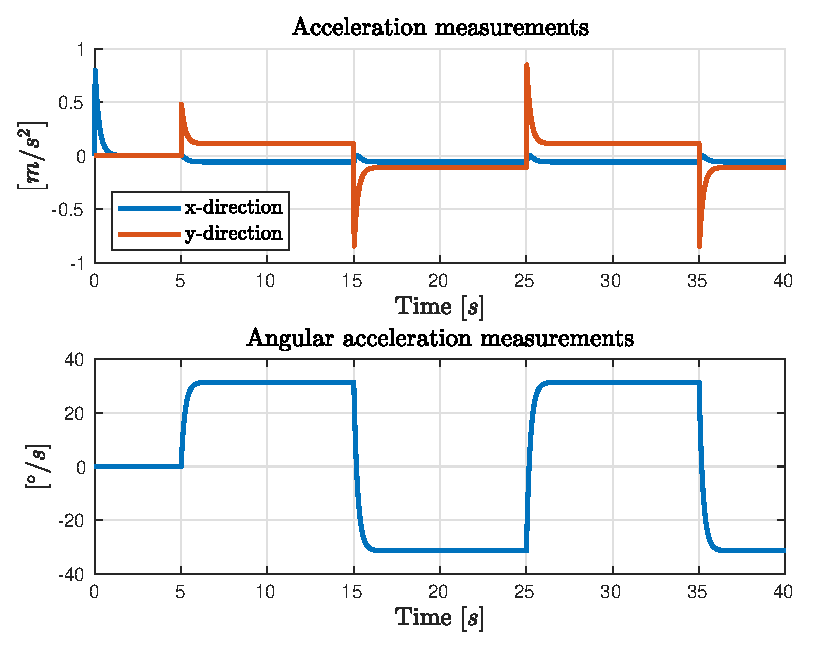
\includegraphics[scale=0.8]{includes/1_measurements_ex1.eps}
	\caption{Mediciones entregadas por los acelerómetros y el giróscopo.} \label{1_measurements_ex1}
\end{figure}

\begin{figure}[ht]
	\centering
	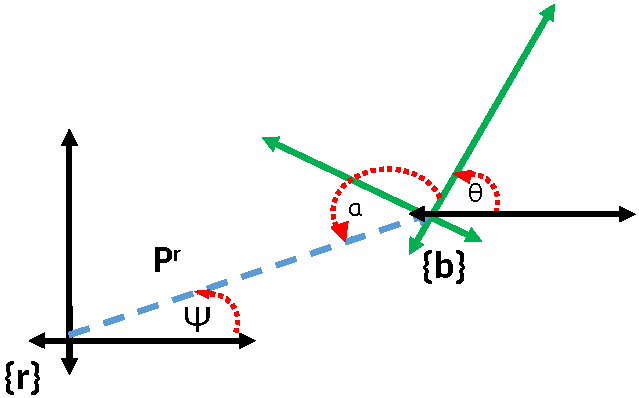
\includegraphics[scale=0.7]{includes/4_sistemas_camara.pdf}
	\caption{Relaciones entre sistemas de referencia y ángulo medido por la cámara abordo de un robot.} \label{4_sistemas_camara}
\end{figure}

\begin{figure}[ht]
	\centering
	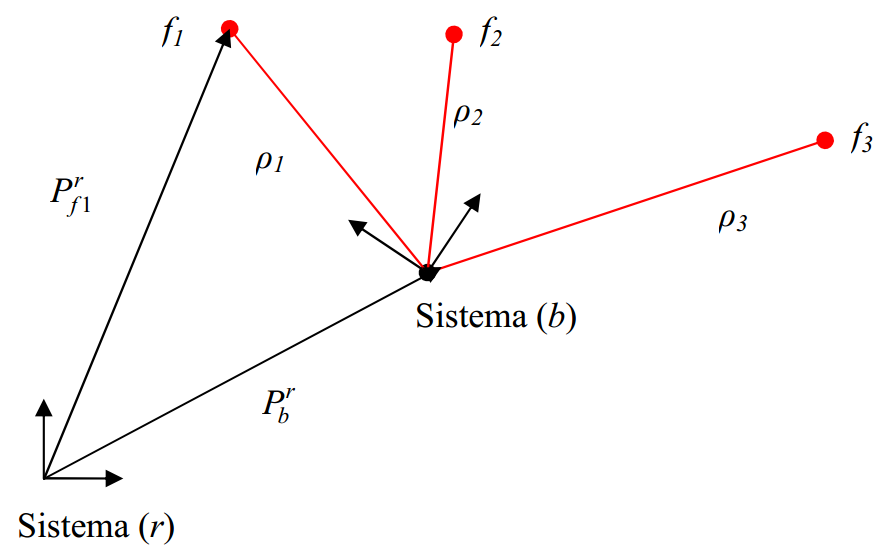
\includegraphics[scale=0.35]{includes/4_sound_sources_diagram.png}
	\caption{Disposición de las fuentes sonoras.} \label{4_sound_sources_diagram}
\end{figure}


La tabla \ref{tabla_ej2} muestra los resultados obtenidos de la aplicación de un algoritmo numérico para determinar el ángulo $\theta$ y su derivada en función del tiempo $t$.

\begin{table}[!ht]
	\centering
	\begin{tabular}{|l|l|l|l|l|}
		\hline
		\multicolumn{1}{|c|}{} & \multicolumn{2}{c|}{\textbf{$\theta_k[\SI{}{\radian}]$}} & \multicolumn{2}{c|}{\textbf{$d\theta_k/dt[\SI{}{\radian\per\second}]$}} \\ \hline
		\multicolumn{1}{|c|}{\textbf{$t_k$}} & \multicolumn{1}{c|}{\textbf{RK1}} & \multicolumn{1}{c|}{\textbf{RK4}} & \multicolumn{1}{c|}{\textbf{RK1}} & \multicolumn{1}{c|}{\textbf{RK4}} \\ \hline
		0.00 & 5.236e-01 & 0.0 & 0.000e+00 &  0.0 \\ \hline
		0.02 & 5.236e-01 & 0.0 & -1.027e-01 & 0.0  \\ \hline
		... &  &  &  &  \\ \hline
		19.92 & 1.082e-04 & 0.0 & 3.342e-04 & 0.0 \\ \hline
		19.94 & 1.149e-04 & 0.0 & 3.063e-04 & 0.0 \\ \hline
	\end{tabular}
	\caption{Resultados obtenidos para RK1 utilizando el set de datos $m=1$, $l=1$, $b=1$, $\theta_0=0.523599$, $\frac{d\theta}{dt}_0=0$ utilizando un paso $h = 0.02$.}
	\label{tabla_ej2}
\end{table}

%---------------------------%
%							%
%	Seccion: Conclusiones	%
%							%
%---------------------------%
\section{Conclusiones}

Se simularon y validaron algoritmos de ..., y se cumplió con el objetivo de ...

%---------------------------%
%							%
%	Seccion: Bibliografía	%
%							%
%---------------------------%
\clearpage
\begin{thebibliography}{10}
	\bibitem{latex} 
	\href{https://tobi.oetiker.ch/lshort/lshort-a5.pdf}{The Not So Short
		Introduction to \LaTeX 2} - Tobias Oetiker - Version 6.3, March 26, 2018.
	\bibitem{Zill} 
	\emph{Ecuaciones diferenciales con problemas de valores en la frontera} - Zill, Dennis G. - Cullen, Michael R. - Thompson 6ta ed. - 2007
	
	\bibitem{Apuntes} 
	\emph{Apuntes del curso Análisis numérico 1 - curso Sassano} - Facultad de Ingeniería - Universidad de Buenos Aires - 2020.
	
\end{thebibliography}

\end{document}
